%What is Giraf?
%What is the point of the project?
\section{Giraf semester project} % (fold)
\label{cha:Giraf semester project}

% chapter Giraf semester project (end)
The following section is about what the Giraf project is, and how it is developed. The information in the section is mostly based on information from the Giraf website\ref{GirafWebsite}.
Giraf is a project that focuses on making digital tablet apps to use as tools for autistic people with limited verbal communication skills. The apps are developed as the main focus of the bachelor projects for several teams of Software students from Aalborg University. The teams work together and coordinates the work between themselves, in collaboration with employees from institutions working with  autistic people. The project has run since 2011, and each year, the students continue where the last year students left off. 
There are already developed many tools, among them both games and a week schedule. However, many of the apps that worked at one point, stopped working after changes in the backend architecture\cite{AppsStatus2019}. 
In the beginning of the semester, the only functioning app was the Week Planner app\cite{AppsStatus2019}. In this App, it is possible to make week schedules. In each schedule there is an entry for every day of the week, see \autoref{fig:WeekPlannerPicture}. 

\begin{figure}[h]
        \begin{center}
            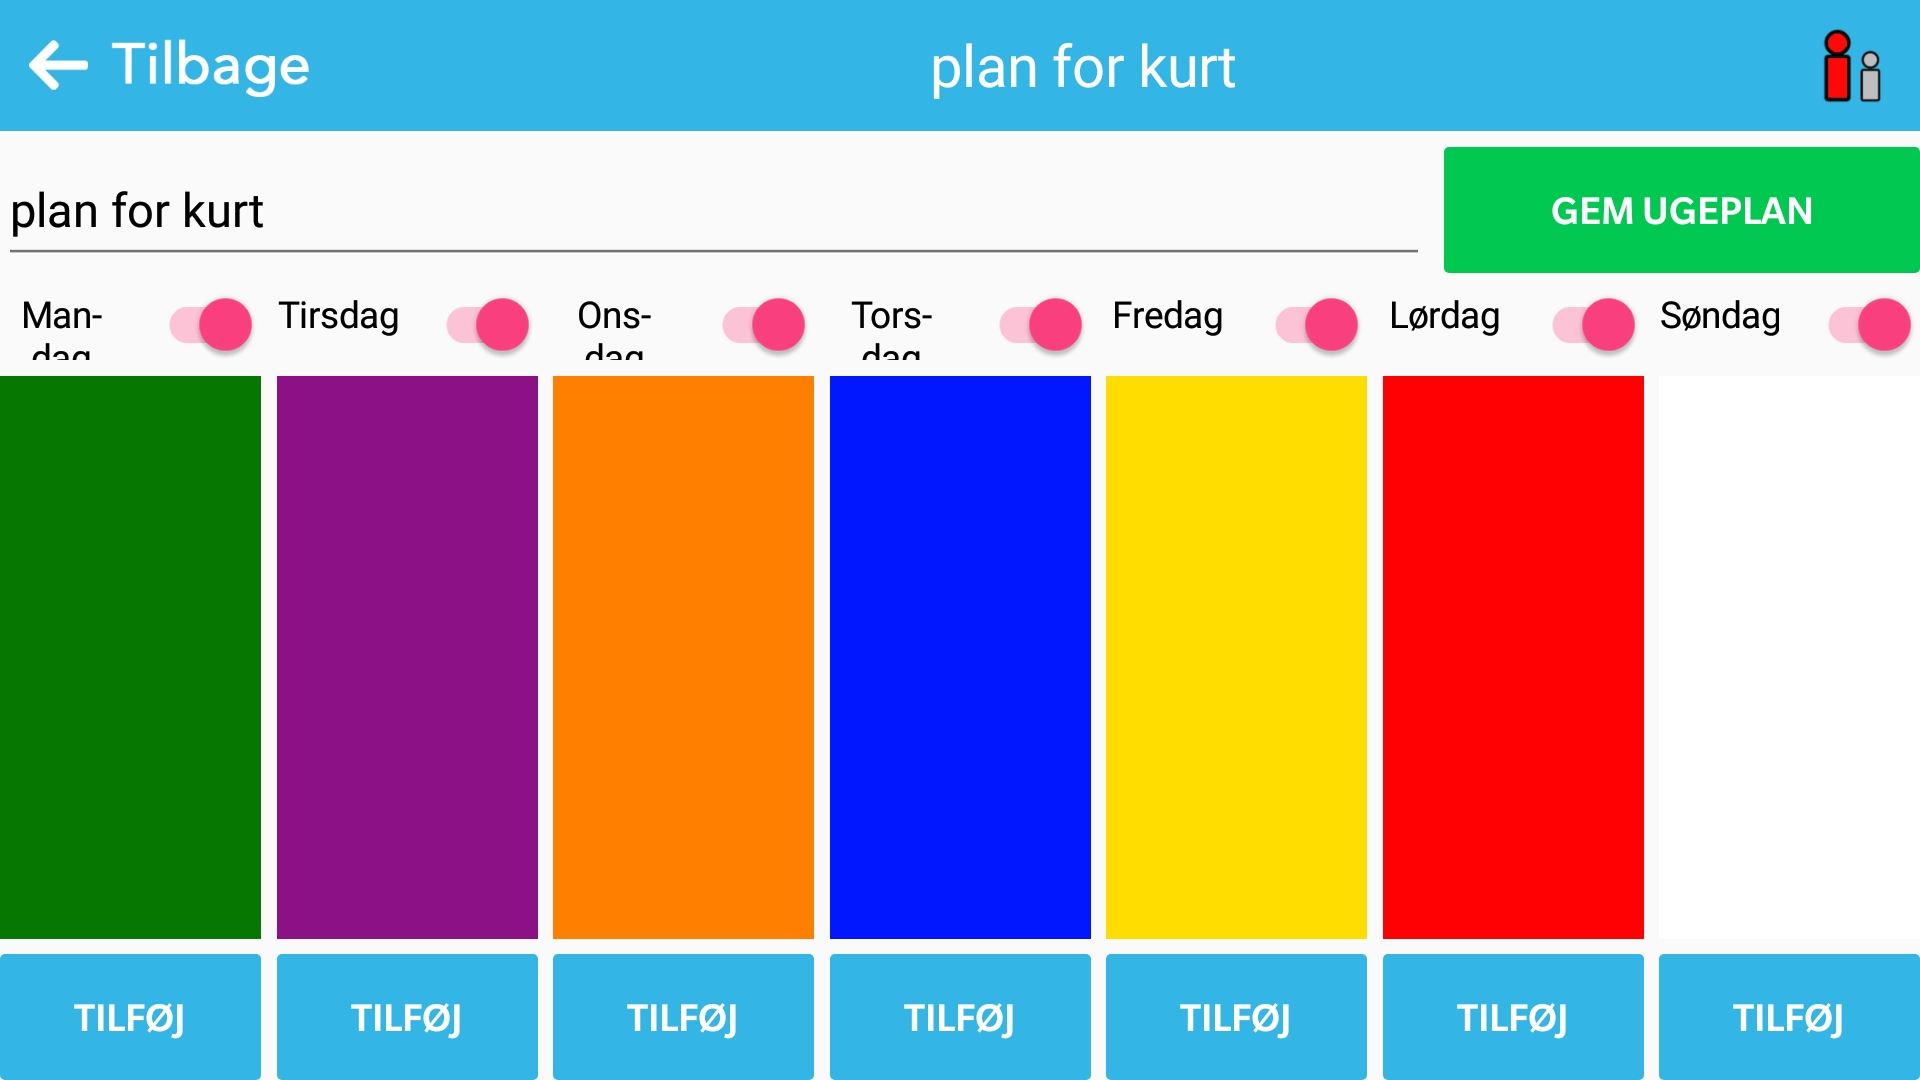
\includegraphics[width=0.95\textwidth]{figures/WeekPlannerPicture}
        \end{center}
        \caption{Weekplanner state at the start of 2019}
        \label{fig:WeekPlannerPicture}
\end{figure}

On each day a series of pictures can be placed. These pictures symbolizes an activity that has to be performed that day, the activities will then be performed from the top down. 
This way of representing activities is a well known approach for showing autistic people what will happen, and is often done using physical pictograms representing every activities. This can however be difficult when a new kind of activity is needed, because a new instance have to be found and cut out every time\cite{AutistTeacher}. In a digital solution, there only need to be constructed a new pictogram, and this can be used as much as nedded, no cutting required. 
The other apps are no longer used, and will therefore not be described. 
The difficulty in having a multi group project run over many years is, that every time a new year starts out, the students has to learn the state of the project, and has only four months to work on it, and then someone else takes over. If the next year has different ideas, or does not get a full picture of the project, it can become messy or, like in the case with the many different apps suddenly not working, ruin things already working. Furthermore, if there is no hard set coding or dokumentation standards, it can be hard to get a clear understanding of what is happening and why.
